\chapter{Propriétés générales des noyaux}

\section{Notations}
	\begin{wrapfigure}[28]{l}{4cm}
	\vspace{-5mm}
	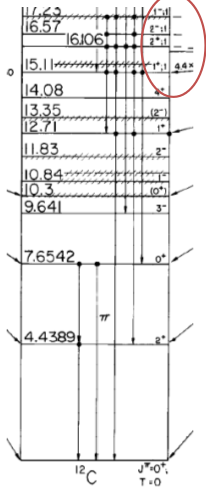
\includegraphics[scale=0.5]{ch3/image1}
	\captionof{figure}{Spectre du $^{12}$C. Entouré l'état d'isopsin $T=1$ et "tout en bas" l'état fondamental
	$J=0^+, T=0$ (petite composante positive).}
	\end{wrapfigure}
On notera un noyau avec $Z$ protons et $N$ neutrons (ou $A=Z+N$)
\begin{equation}
^A _ZX_N\qquad\text{ou}\qquad ^A _ZX\qquad\text{ou}\qquad ^A X
\end{equation}
Par exemple, $^7 _3Li_4, Z=3,N=4$ est noté en pratique $^7$Li. De même, 
$^{12} _C C_6,Z=6,N=6$ est noté $^{12}$C. On parlera de bon nombres quantiques \textbf{exacts} 
\begin{itemize}
\item[$\bullet$] Le spin total $J : [H,J^2]=0$ (invariance par rotation)
\item[$\bullet$] Projection du spin : $J_z : [H, J_z]  = 0$
\item[$\bullet$] Parité $\pi : [H,P] = 0$ (invariance par réflexion
\end{itemize}\

Il y a également le bon nombre quantique \textbf{approché}, l'isospin $T : [H,T^2]\approx0$. Nous noterons
également les niveaux $E, J^p(T)$.






\section{Masses et énergies de liaison}
Il existe deux types de masses qui sont toutes deux importantes pour déterminer la stabilité des noyaux : la masse
atomique et nucléaire. Celles-ci diffèrent par la masse des électrons et des énergies de liaison et leur différence
est souvent négligeable. \\

La \textbf{masse atomique} $M(A,Z)$ ou $M(^AX)$ a pour unité l'unité de masse atomique uma définie par 
\begin{equation}
1\ uma \approx 931.4940\ MeV/c^2
\end{equation}
à partir de la masse d'un atome de $^{12}$C (M($^{12}$C) = 12\ uma). Pour le proton, le neutron et l'électron :
\begin{equation}
m_p = 1.007\ 276\ 467\ uma,\qquad m_n = 1.008\ 664\ 916\ uma, \qquad m_e = 5.485\ 799\ 09 \times 10^{-4}\ uma
\end{equation}

On utilise souvent (dans les table, car plus facile à mesurer) l'\textbf{excès de masse} défini par
\begin{equation}
\Delta (A,Z) = [M(A,Z) - A]\ \text{uma}
\end{equation}
Par définition $\Delta(^{12}C)=0$.

\begin{center}
	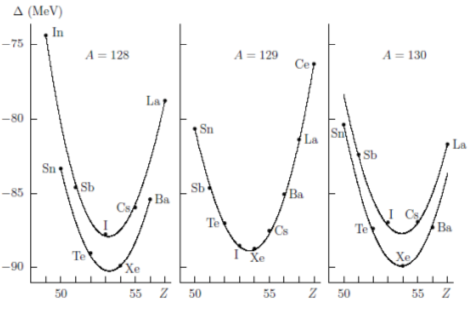
\includegraphics[scale=0.5]{ch3/image2}
	\captionof{figure}{Les valeurs sont négatives car la masse du noyau est inférieur à la somme des masses individuelles. Il y a des
différences entre les valeurs de $A$ pair et impair. Si $A$ est impair, un des deux doit être pair et l'autre
impair. Mais si la somme $A=N+Z$ est paire on peut avoir $N, Z$ soit paire soit impair (noyaux pair-pair ou
impair-impair). L'excès de masse constant justifie cette forme parabolique.}
\end{center}\ 

Les \textbf{masses nucléaires} $m(A,Z)$ ou $m(^AX)$ sont reliée à la masse atomique par
\begin{equation}
m(A,Z) = M(A,Z) - Zm_e + \dfrac{B_e(Z)}{c^2}
\end{equation}
où $B_e(Z)$ est l'énergie de liaison électronique valant à peu près $15.7*Z^{7/3}$ eV (négligeable). La masse
nucléaire est donne la masse atomique diminuée de "tout ce qui concerne les électrons" (soit leur masse et 
énergie de liaison).\\

	\begin{wrapfigure}[8]{l}{8.5cm}
	\vspace{-5mm}
	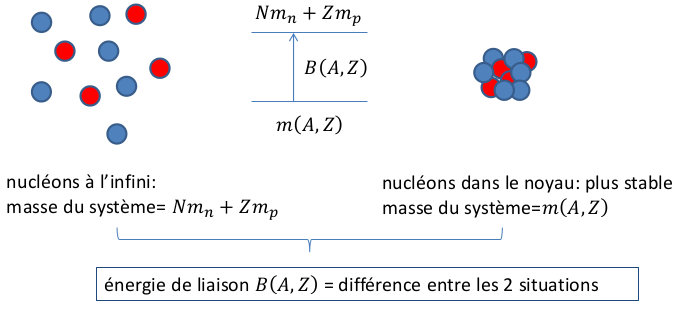
\includegraphics[scale=0.35]{ch3/image3}
	\captionof{figure}{ }
	\end{wrapfigure}


L'\textbf{énergie de liaison nucléaire} est définie
\begin{equation}
\begin{array}{ll}
B(A,Z) &= [Nm_n + Zm_p-m(A,Z)]c^2 \\ 
&= N\Delta (n) + N\Delta(p) - \Delta(A,Z)\end{array}
\end{equation}
Cette énergie $B$ est positive pour tous les noyaux connus, c'est-à-dire qu'ils ne se désintègrent pas en 
$N$ neutrons et $Z$ protons.\\


\begin{center}
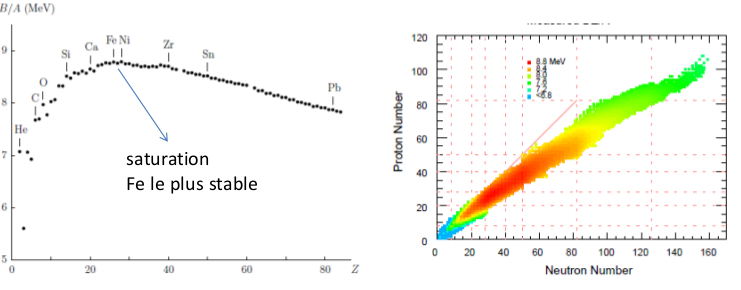
\includegraphics[scale=0.45]{ch3/image4}
\captionof{figure}{ }
\end{center}

De façon presque systématique, on peut dire que
\begin{equation}
\dfrac{B(A,Z)}{A} \approx (8.3 \pm 0.5)\ \text{MeV}
\end{equation}
Ceci est illustré sur la figure ci-dessus. A partir de $Z=20$, 8MeV est vraiment l'énergie moyenne pour l'énergie
de masse (s'il y a un chiffre à retenir, c'est lui). A gauche du fer, on gagne de l'énergie de liaison
si on ajoute des nucléons : production d'énergie dans les étoiles, il s'agit de la fusion. On ajoute en 
effet aux éléments léger un proton ou une particule alpha et on gagne en liaison ce qui produit un rayonnement. Le
$^4$He sort de cette tendance, étant très lié : il s'agit de la particule $\alpha$ qui possède une grande énergie
de liaison (7.1 MeV)(par contre le deuton est lui très peu stable (1.1 MeV)).


\subsection{Formule de masse : modèle de la goutte liquide}
Le modèle de la goutte liquide est une paramétrisation empirique. Il s'agit de considérer que le  noyau est une
goutte liquide possédant certaines propriétés. Il s'agit d'un modèle macroscopique qui ne tient pas compte
des effets quantiques mais qui permet de pas mal décrire l'énergie de liaison (pour les noyaux stables!).\\

Selon ce modèle, l'énergie de liaison totale est donnée par
\begin{equation}
B(A,Z) = a_VA - a_SA^{2/3}-\dfrac{a_cZ(Z-1)}{A^{1/3}}-\dfrac{a_a(N-Z)^2}{A}+\delta
\end{equation}
Cette relation permet de donner un ordre de grandeur aux énergies de liaison. Il contient cinq termes
\begin{enumerate}
\item Terme de volume : plus il y a de nucléons, plus $B$ grandit. On considère ici que chaque nucléon 
interagit avec tous les autres.
\item Terme de surface : il s'agit de la première correction. Les nucléons à la surface interagissent 
moins que ceux à l'intérieur qui ont "plus de voisins". La matière nucléaire est incompressible, le volume d'un
noyau est proportionnel au nombre de nucléon $A$. Ceci signifie que le rayon du noyau est proportionnel à 
$A^{1/3}$ et donc que $S\propto A^{2/3}$.
\item  Terme coulombien incluant chaque parie de protons
\item Terme d'asymétrie, proportionnel à la différence entre les deux (le principe de \textsc{Pauli} 
favorise en effet $Z=N$).
\item Énergie d'appariement (favorise les paires de nucléons).
\end{enumerate}\ 

	\begin{wrapfigure}[7]{l}{6cm}
	\vspace{-10mm}
	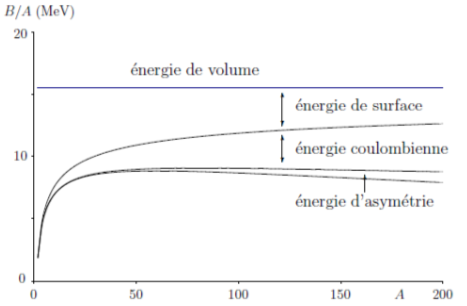
\includegraphics[scale=0.35]{ch3/image5}
	\captionof{figure}{ }
	\end{wrapfigure}
Tous ces paramètres sont obtenus à partir d'ajustements. Il existe des formules plus compliquée pour des 
noyaux instables (d'autres effets sont pris en compte). En utilisant l'expression de $B(A,Z)$, on retrouve bien la dépendance en 
$Z^2$ à $A$ constant. Parmi les noyaux stables, 166 noyaux sont pair-pair, 55 pair-impair et 4 
impair-impair ($^2$H, $^6$Li, $^{10}$B et $^{14}$N).

\newpage
Il est possible de retrouver la parabole de masse à partir de ce modèle (soit la variation de fonction de $Z$, à
$A$ fixe). Petit calcul d'optimisation
\begin{equation}
\left.\begin{array}{ll}
B(A,Z) &= [Nm_n + Zm_p-m(A,Z)]c^2 \\
B(A,Z) &= a_VA - a_SA^{2/3}-\dfrac{a_cZ(Z-1)}{A^{1/3}}-\dfrac{a_a(N-Z)^2}{A}+\delta
\end{array}\right\} \Rightarrow 
\dfrac{dm}{dZ} = 2Z\frac{a_c}{A^{1/3}}-\dfrac{2(A-2Z)a_a}{A} = 0
\end{equation}
où nous avons fait les hypothèses que $m_n\approx m_p$ et $2Z-1\approx 2Z$. On en déduit que 
\begin{equation}
Z_{min} \approx \frac{A}{2}\dfrac{1}{1+\left(\frac{a_C}{4a_a}\right)A^{2/3}} \approx
\frac{A}{2}\dfrac{1}{1+0.0078A^{2/3}}
\end{equation}
Le rapport $Z_{min}/A$ diminue quand $A$ augmente (s'écarte de 1/2) :
\begin{equation}
m(A,Z) \approx m(A,Z_{min}) +c\times(Z-Z_{min})^2 + \dots
\end{equation}
On retrouve bien la forme parabolique. 
\begin{center}
	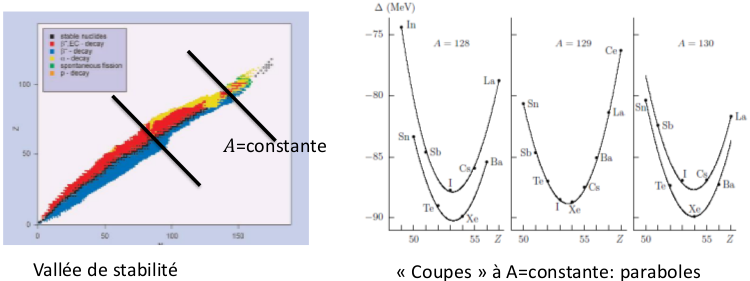
\includegraphics[scale=0.5]{ch3/image6}
	\captionof{figure}{A gauche, les points noirs représentent la vallée de la stabilité. En rouge il s'agit
	des éléments riches en protons et en bleus ceux riches en neutrons. En faisant une coupe en se plaçant sur 
	un des points noir, on obtient les paraboles représentées à droite.}
\end{center}


Intéressons-nous aux \textbf{énergies de séparation}
\begin{itemize}
\item[$\bullet$] Un neutron
\begin{equation}
S_n = (m(A-1,Z)+m_n-m(A,Z))c^2 = B(A,Z)-B(A-1,Z)
\end{equation}
\item[$\bullet$] Deux neutrons
\begin{equation}
S_n =  B(A,Z)-B(A-2,Z)
\end{equation}
\item[$\bullet$] Un proton
\begin{equation}
S_P = B(A,Z) - B(A-1, Z-1)
\end{equation}
\end{itemize}\ 

Il s'agit de l'énergie qu'il faut fournir au système pour enlever un neutron (proton). Trois cas peuvent se
présenter
\begin{enumerate}
\item $S > 0$ : le noyau est stable en particules
\item $S < 0$ : le noyau est instable en particules
\item $S = 0$ : le noyau est à la limite de stabilité (\textit{driplines})
\end{enumerate}\ 

	\begin{wrapfigure}[11]{l}{6cm}
%	\vspace{-5mm}
	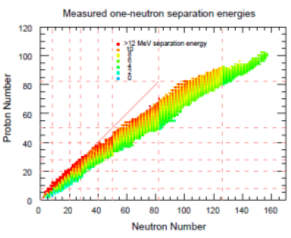
\includegraphics[scale=0.5]{ch3/image7}
	\captionof{figure}{ }
	\end{wrapfigure}

Lorsque l'on "coupe" un noyau, la masse peut être supérieure ou inférieure. Dans le cas où la masse est plus 
grande, le noyau initial était plus stable car il possédait une masse plus petite. Dans le cas où la masse
coupée est plus petite, le noyau initial est instable et il aura tendance à émettre un neutron. Sur le graphique
ci-contre, il s'agit d'un code couleur pour les énergies de séparation d'un neutron. Le \textit{vert} et le
\textit{bleu} correspondent à de petites énergies de liaison. Le neutron est donc de moins en moins lié et il
faut de moins en moins d'énergie pour l’éliminer et converger vers une situation stable.



\section{Stabilité du noyau}
Il existe principalement deux types d'instabilité : l'instabilité en \textbf{particule} et par 
\textbf{émission $\beta$}. Dans le premier cas\footnote{Il s'agit du cas précédemment discuté ou le nombre de
nucléons changeait.}, $A$ change et cette instabilité est en générale très courte ($\approx 10^{-21}$s) alors que
dans le second cas\footnote{Les atomes à l'extrémité de la valée de la stabilité sont instable par émission 
$\beta$.} $A$ est constant (mais $N,Z$ changent) et les durées de vie sont variables ($10^{-6}$s à $10^{15}$ ans).\\

La \textit{stabilité en particule} s'obtient s'il n'existe pas de sous-système (2,3,4, \dots particules) dont
l'énergie totale est plus basse. Considérons un noyau $(A,Z)$ et différents mode de dissociation
\begin{equation}
(A,Z)\to (A_1,Z_1)+(A_2,Z_2)
\end{equation}
où $A = A_1+A_2$ et $Z=Z_1+Z_2$. Le noyau sera stable en particules si
\begin{equation}
\begin{array}{ll}
m(A,Z)&< m(A_1,Z_1)+m(A_2,Z_2)\qquad\forall(A_1,Z_1)\\
B(A,Z)&> B(A_1,Z_1)+B(A_2,Z_2)\qquad\forall(A_1,Z_1)
\end{array}
\end{equation}
Le \textit{slide 43}  donne quelques arrangement possible pour la dissociation du $^7$Li. En regardant les 
différents cas on se rend compte qu'aucune n'est possible : le $^7$Li est donc stable en particules. On remarque
ici que toutes les différences de masses étaient négatives ce qui implique la stabilité (masse initiale plus 
petite que la masse finale).\\

	\begin{wrapfigure}[9]{r}{7cm}
%	\vspace{-5mm}
	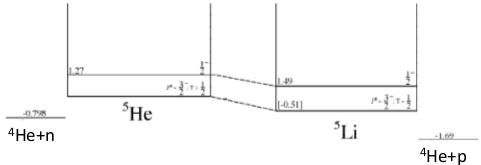
\includegraphics[scale=0.45]{ch3/image8}
	\captionof{figure}{ }
	\end{wrapfigure}
Si cette différence est par contre un nombre \textbf{positif}, le noyau est instable en particules. C'est le
cas pour le $^8$Be
\begin{equation}
m(^8Be)-2*m(^4He) = 0.092\ \text{MeV}
\end{equation}
La masse du $^4$He est plus petite car le rapport $B/A$ est grand, le noyau est instable et possède une durée de 
vie de $10^{-16}$s. Le noyau $^8$Be est donc en dehors de la vallée de stabilité. De même, il n'existe pas de
noyaux stables pour $A=5$. Regardons les deux dissociations suivantes
\begin{equation}
^5He \to \alpha+n,\qquad\qquad\qquad ^5Li\to\alpha+p
\end{equation}
En calculant leurs différences de masses
\begin{equation}
m(^5He)-m(^4He)-m(n) = 0.0798\ \text{MeV},\qquad 
m(^5Li)-m(^4He)-m(p) = 1.69\ \text{MeV}
\end{equation}
On voit donc qu'ils ont une masse initial plus grande que les produits de dissociation : $^5$He et $^5$Li 
n'existent pas, il se désintègrent quasi directement. Le fondamental apparaît donc comme une résonance
(temps de vie de $\approx 10^{-20}$s).\\


	\begin{wrapfigure}[9]{r}{6cm}
	\vspace{-5mm}
	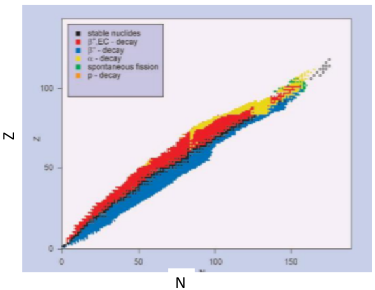
\includegraphics[scale=0.45]{ch3/image9}
	\captionof{figure}{ }
	\end{wrapfigure}
	
Il existe d'autres types de décroissance
\begin{itemize}
\item[$\bullet$] Radioactivité $\alpha$ : $m(A,Z) - m(A-4,Z-2)-m_\alpha > 0$ pour $A\gtrsim 150$
\item[$\bullet$] Fission (symétrique) : $M(A,Z)-2m(A/2,Z/2) >0$ pour $A\gtrsim 190$
\item[$\bullet$] Radioactivité $\beta$ : pour $A$ donné, un seul $Z$ est stable
\begin{itemize}
\item $\beta^-$ (neutron converti en proton et émission d'un électron) : $(A,Z)\to (A,Z+1)+e^-+\bar{\nu}$
\item $\beta^+$ (proton converti et neutron et émission d'un positron) : $(A,Z)\to (A,Z-1)+e^++\nu$
\end{itemize}
\item[$\bullet$] Radioactivités \textit{exotiques} : 2$p$, $^{14}$C, double $\beta$, \dots
\end{itemize}\

Sur la figure ci-dessus à droite, en \textit{noir} sont représentés les noyaux stables, en \textit{bleu}
ceux qui ont un excès de neutron (et donc désintégration $\beta^-$), en \textit{rouge} ceux qui ont un
excès de proton (et donc désintégration $\beta^+$). Dans la zone des noyaux lourds, en retrouve en 
\textit{jaune} la désintégration $\alpha$. Il faut en effet être dans la zone des noyaux lourd pour 
gagner de l'énergie (ou perdre de la masse, c'est identique) et émettre de $\alpha$. Les quelques points
\textit{verts} représentent la fission.\\

	\begin{wrapfigure}[6]{l}{4.5cm}
	\vspace{-8mm}
	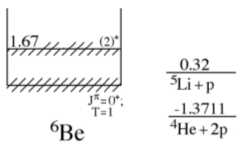
\includegraphics[scale=0.45]{ch3/image10}
	\captionof{figure}{ }
	\end{wrapfigure} 
Regardons deux radioactivités \textit{exotiques}, en commençant par la désintégration $2p$ dans le $^6$Be. 
Celui-ci est stable par rapport à $^5$Li+$p$ mais instable par rapport à $^4He+p+p$ : il est donc stable
par rapport à la désintégration en un proton, mais instable par rapport à celle à deux protons.\\

Un autre cas un peu spécial est la radioactivité double $\beta$, la décroissante $\beta$ étant défavorisée
\begin{equation}
^{48}Ca\ (Z=20) \to ^{48}Ti\ (Z=22) + 2e^- + 2\bar\nu
\end{equation}
Ce phénomène est cependant peu fréquent, la durée de vie du $^{48}$Ca étant de $5*10^{19}$ ans. 

\subsection{Durée de vie des noyaux}
Le graphique ci-dessus résume ce que nous venons de voir, en terme de durée de vie. Notons que la droite
$N=Z$ n'est vraie que jusqu'à 20 neutrons.
\newpage
\begin{center}
	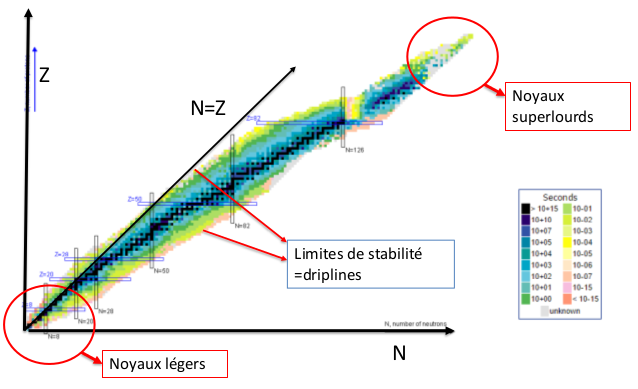
\includegraphics[scale=0.55]{ch3/image11}
	\captionof{figure}{ }
\end{center}

\section{Nombre "magiques"}
	\begin{wrapfigure}[11]{l}{6cm}
%	\vspace{-8mm}
	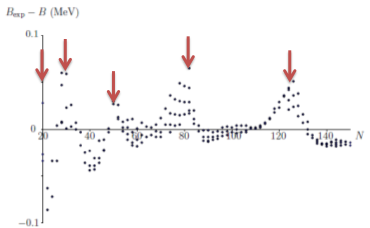
\includegraphics[scale=0.45]{ch3/image12}
	\captionof{figure}{ }
	\end{wrapfigure} 
Nous avons utilisé un modèle macroscopique (modèle de la goutte liquide) pour déterminer l'énergie de liaison. 
En comparant ces résultats théoriques avec les expérimentaux, il y a des différences importantes pour 
$N=2,8,20,28,50,82,126$. On appelle ces nombres les \textit{nombres magiques} qui possèdent des propriétés 
remarquables au niveau de l'énergie de liaison du rayon et de l'énergie d'excitation. Notons qu'il existe
aussi des nombres \textit{doublements magiques} qui, comme les \textit{magiques} doivent être expliqués par 
des modèles nucléaires (effets quantiques : modèle en couche).


\section{Densité et rayons nucléaires}
	\begin{wrapfigure}[11]{r}{5cm}
%	\vspace{-8mm}
	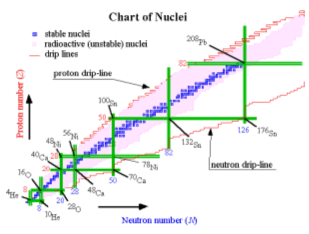
\includegraphics[scale=0.45]{ch3/image13}
	\captionof{figure}{ }
	\end{wrapfigure}
Il existe principalement quatre types de noyaux
\begin{enumerate}
\item \textit{Exotiques} : situés près de la limite de stabilité ($S_n=0,S_p=0$ : \textit{drip lines})
\item \textit{Halo} : Rayon beaucoup plus grand que prédit par la loi en $A^{1/3}$
\item \textit{Transuraniens} : charge $Z > 92$ (Uranium). Ils n'existent pas dans la nature et sont produits
en laboratoire (actuellement jusque $Z=118$).
\item \textit{Superlourds} : hypothétiques, proche de $Z=126$ le nombre magique suivant).
\end{enumerate}

\newpage
\section{Densité et rayons nucléaires}
Peu de notes dans cette section\footnote{NOTES!!}. Il existe deux types de densité ([$L^{-3}$])
\begin{enumerate}
\item \textbf{Matière} (masse)
\begin{equation}
\rho_m(\vec{r}) = \bra{\Psi^{JJ\pi}}\sum_{i=1}^A\delta(\vec{r}-\vec{r}_i)\ket{\Psi^{JJ\pi}}
\end{equation}
\item \textbf{Charge}
\begin{equation}
\rho_c(\vec{r}) = \bra{\Psi^{JJ\pi}}\sum_{i=1}^Z\delta(\vec{r}-\vec{r}_i)\ket{\Psi^{JJ\pi}} =
\bra{\Psi^{JJ\pi}}\sum_{i=1}^A\left( \frac{1}{2}-t_{iz} \right)\delta(\vec{r}-\vec{r}_i)\ket{\Psi^{JJ\pi}}
\end{equation}
\end{enumerate}\ 

Ces densité vérifient les relations $\int \rho_m(\vec{r})d\vec{r}=A$ et $\int \rho_c(\vec{r})d\vec{r}=Z$ mais
il s'agit également de fonctions paires $\rho(\vec{r})=\rho(-\vec{r})$. L'application de l'opérateur de 
parité $P$ donne $P\delta(\vec{r}-\vec{r}_i)P=\delta(\vec{r}+\vec{r}_i)$.\\

Il est possible d'exprimer ces densités selon un \textbf{développement en multipoles} (rouge)
\begin{equation}
\rho(\vec{r}) = \sum_\lambda P_\lambda(\cos\theta)\rho_\lambda(r)
\end{equation}
où $\lambda$ est pair et compris entre 0 et $2J$. Si $J=0$ ou $J=1/2$, $\rho(\vec{r})=\rho_0(r)$, les densités
sont alors sphériques. \\

Autre donnée intéressantes, les \textbf{rayons carrés} pour ces deux densités. Pour la matière
\begin{equation}
\langle r^2\rangle_m = \frac{1}{A}\sum_i r_i^2 = \frac{1}{A}\int \rho_m(\vec{r})r^2dr
\end{equation}
Celle-ci ne dépend que de $\rho_0$. Pour la charge :
\begin{equation}
\langle r^2\rangle_c = \frac{1}{Z}\sum_i r_i^2 = \frac{1}{Z}\int \rho_m(\vec{r})r^2dr
\end{equation}

Si $T=0$, alors $\langle r^2\rangle_c=\langle r^2\rangle_m$.\\


Il est courant de considérer la distribution de \textsc{Fermi} comme densité $\rho(r)$
\begin{equation}
\rho(r) = \frac{\rho_0}{1+\exp\left(\frac{r-R}{a}\right)}
\end{equation}
où $a$ est la diffusivité ($\approx 0.5$ fm) et $R$ la portée. Pour une diffusivité nulle ($a=0$), on trouve
$\langle r^2\rangle = \frac{3}{5}R^2$. Le volume est également proportionnel à $A$. Nous avons en effet (rouge)
\begin{equation}
R = r_0A^{1/3}
\end{equation}
où $r_0 \approx$ 1.24 fm. 
\begin{center}
	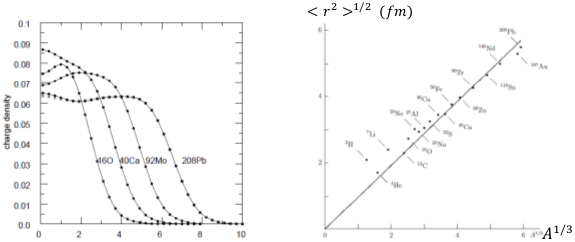
\includegraphics[scale=0.55]{ch3/image14}
	\captionof{figure}{ }
\end{center}

Ce faisait, la loi en $A^{1/3}$ est généralement bien vérifiée (voir graphique ci-dessus),
seuls les noyaux exotiques à \textit{halo} s'éloignent de cette systématique :
\begin{itemize}
\item[$\bullet$] $^6$He : $\sqrt{\langle r^2\rangle} \approx 2.50$ fm, $r_0A^{1/3} = 2.25$ fm.
\item[$\bullet$] $^11$Li : $\sqrt{\langle r^2\rangle} \approx 3.50$ fm, $r_0A^{1/3} = 2.75$ fm.
\end{itemize}\ \\

	\begin{wrapfigure}[10]{r}{7cm}
	\vspace{-5mm}
	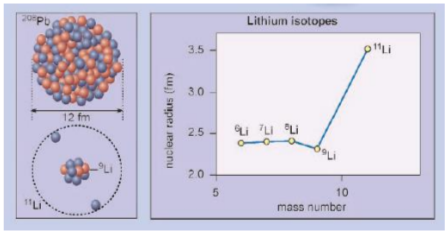
\includegraphics[scale=0.45]{ch3/image15}
	\captionof{figure}{ }
	\end{wrapfigure}
Attardons-nous quelque peu sur le $^{11}$Li. Considérons les rayons expérimentaux pour différents types de
Li et remarquons directement que le $^{10}$Li n'existe pas, celui-ci se désintègre directement. Entre 
$^9$Li et $^{11}$Li, l'écart est très important. Cette grand différence vient du fait que $^{11}$Li est à la
limite de la stabilité : l'énergie de liaison est toute petite et le rayon est donc grand. L'énergie de 
séparation de deux neutrons est également très petite, car les niveaux sont très proches. Il est possible de
comprendre ça en suivant un raisonnement très qualitatif en supposant qu'il n'y a qu'un seul neutron à 
l'extérieur? Il existe un potentiel $V(r)$ entre ces deux particules. Selon l'équation de \textsc{Schrödinger}
\begin{equation}
-\frac{\hbar^2}{2\mu}\psi'' + V(r)\psi = E\psi
\end{equation}
où $E=-\delta_m$, l'énergie de liaison. On ne connaît pas $V$, mais il est nul à grande distance. L'énergie étant
négative, la solution sera exponentielle. En supprimant l'exponentielle divergente
\begin{equation}
\psi \Rightarrow \exp(-kr)
\end{equation}
Faisons maintenant une grossière approche en supposant que ceci n'est pas valable à grande distance mais partout
et calculons-en le rayon carré moyen 
\begin{equation}
\langle r^2\rangle = \dfrac{\int |\psi|^2r^2 dr}{\int |\psi|^2 dr}
\end{equation}
En utilisant notre $\psi$ et par changement de variable, on voit que 
\begin{equation}
\langle r^2\rangle \propto 1/k^2
\end{equation}
Cette simple formule nous dit que quand l'énergie de liaison diminue, le rayon carré moyen (soit la taille du 
noyau) augmente. Ici le raisonnement tenu est très simple, mais qualitativement tout à fait valable.

\newpage
\section{Moments multipolaires}
Ces moments sont intimement liés à la déformation du noyau et sont utilisés pour tester les modèles 
nucléaires\footnote{Pas de notes sur cette dernière section, la précédente ok.}

\subsection{Moment quadrupolaire électrique}
Par définition ([e.fm$^2$])
\begin{equation}
Q = \sqrt{\dfrac{16\pi}{5}}e\bra{\Psi^{JJ\pi}}\sum_{i=1}^Z r_i^2Y_2^0(\Omega_i)\ket{\Psi^{JJ\pi}}
\end{equation}
Si $J<1$, alors par le théorème de \textsc{Wigner-Eckart} pour un OTI de rang 2, on en déduit que $Q=0$. Pour 
l'interprétation, il faut savoir que
\begin{equation}
r^2P_2(\cos\theta) = \frac{1}{2}(2z^2-x^2-y^2)
\end{equation}
Trois cas sont donc possibles
\begin{description}
\item[Q>0] Noyau allongé (\textit{prolate})
\item[Q<0] Noyau aplati
\item[Q=0] Noyau sphérique
\end{description}\ 

On peut ré-écrire l'élément de matrice dans le formalisme de l'isospin
\begin{equation}
\bra{\Psi^{JJ\pi}}\sum_{i=1}^Z r_i^2Y_2^0(\Omega_i)\ket{\Psi^{JJ\pi}} =
\bra{\Psi^{JJ\pi}}\sum_{i=1}^A \left(\frac{1}{2}-t_{iz}\right) r_i^2Y_2^0(\Omega_i)\ket{\Psi^{JJ\pi}}
\end{equation}
Par les propriétés du moment quadrupolaire, il est possible d'énoncer une définition alternative
\begin{equation}
\bra{\Psi^{JJ\pi}}\sum_{i=1}^Z r_i^2Y_2^0(\Omega_i)\ket{\Psi^{JJ\pi}} = \sqrt{\dfrac{4\pi}{5}}\int
\rho_{c,2}(r)r^2dr
\end{equation}
Le moment quadrupolaire est donné par le terme $\lambda=2$ de la densité de charge.

\subsection{Moment dipolaire magnétique}
Par définition
\begin{equation}
\mu = \sqrt{\dfrac{4\pi}{3}}\bra{\Psi^{JJ\pi}}M_0\ket{\Psi^{JJ\pi}}
\end{equation}
où $\vec{M} = \mu_N\sum_i(g_i\vec{l_i}+g_{si}\vec{s_i})$ avec $\mu_N=\frac{e\hbar}{m_Nc}$ le 
magnéton de \textsc{Bohr}, $g_s(n)=-3.82, g_s(p)=5.58$ les rapports gyromagnétiques et 
$g_l(i) = \frac{1}{2}-t_{iz}=0$ pour le neutron et 1 pour le proton. Si $J=0$ alors $\mu=0$ 
($\vec{M}$ est alors un opérateur de rang 1). Les moments quadrupolaire électrique et dipolaire 
magnétique sont utilisés pour tester les modèles nucléaires